\SourceLeaf{200}\clearpage
\begin{center}[ZUR THEORIE DER GERADEN LINIE UND DER EBENE.]\end{center}


\begin{center}[1.]\end{center}


[\textls{Euklids Elemente} Buch I. Lehrsatz 7: »Sind von den Endpunkten einer Geraden nach
einem Punkt ausserhalb zwei Gerade gezogen, so ist es unmöglich, von diesen
Endpunkten aus nach einem andern Punkt auf derselben Seite jener Geraden zwei
Gerade zu ziehen, die den ersten beziehungsweise gleich sind.]

\begin{center}
\begin{minipage}[b]{.42\linewidth}\centering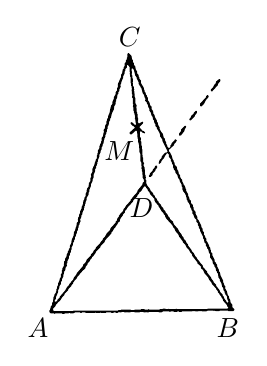
\begin{tikzpicture}[x=0.00594059cm,y=-0.00594059cm]
\fill[even odd rule] (369,402) -- (367,402) -- (359,410) -- (359,413) -- (355,418) -- (355,422) -- (356,423) -- (359,422) -- (366,413) -- (367,409) -- (370,404) -- cycle
(392,370) -- (390,370) -- (386,374) -- (386,376) -- (381,380) -- (379,385) -- (377,387) -- (377,389) -- (378,390) -- (380,390) -- (388,382) -- (389,379) -- (393,374) -- (393,371) -- cycle
(416,336) -- (415,336) -- (413,338) -- (412,341) -- (400,354) -- (400,359) -- (401,360) -- (403,360) -- (408,355) -- (412,347) -- (418,340) -- (418,338) -- cycle
(442,302) -- (440,302) -- (434,307) -- (433,311) -- (430,314) -- (427,320) -- (423,324) -- (423,327) -- (424,328) -- (426,328) -- (427,326) -- (433,320) -- (433,319) -- (437,316) -- (438,312) -- (443,306) -- (443,303) -- cycle
(246,246) -- (244,248) -- (244,255) -- (243,256) -- (243,259) -- (241,262) -- (241,265) -- (238,269) -- (238,274) -- (236,277) -- (236,280) -- (234,282) -- (233,289) -- (231,292) -- (231,296) -- (224,312) -- (224,319) -- (222,321) -- (222,326) -- (219,330) -- (219,334) -- (215,341) -- (215,344) -- (212,351) -- (212,355) -- (209,359) -- (209,362) -- (208,363) -- (206,374) -- (203,381) -- (203,384) -- (201,387) -- (201,389) -- (199,393) -- (199,398) -- (197,400) -- (196,407) -- (193,411) -- (194,413) -- (194,416) -- (193,417) -- (192,424) -- (189,428) -- (189,434) -- (188,435) -- (188,438) -- (186,441) -- (186,443) -- (184,445) -- (184,450) -- (181,455) -- (181,460) -- (180,461) -- (180,464) -- (179,465) -- (179,471) -- (176,475) -- (176,478) -- (175,479) -- (173,487) -- (171,490) -- (171,492) -- (169,494) -- (169,501) -- (166,506) -- (167,510) -- (165,514) -- (165,520) -- (162,524) -- (161,532) -- (158,536) -- (158,538) -- (157,539) -- (157,543) -- (155,547) -- (155,552) -- (152,556) -- (152,559) -- (150,562) -- (149,570) -- (148,571) -- (148,573) -- (146,575) -- (146,579) -- (143,585) -- (143,588) -- (141,592) -- (141,595) -- (139,598) -- (139,601) -- (138,602) -- (139,606) -- (136,609) -- (135,617) -- (134,618) -- (132,626) -- (130,629) -- (129,637) -- (125,646) -- (124,653) -- (121,659) -- (121,663) -- (119,665) -- (119,668) -- (117,670) -- (117,672) -- (114,678) -- (114,681) -- (111,686) -- (111,690) -- (109,692) -- (108,702) -- (105,707) -- (105,710) -- (104,711) -- (104,717) -- (102,719) -- (102,725) -- (99,730) -- (99,732) -- (96,739) -- (96,742) -- (94,746) -- (94,749) -- (92,752) -- (92,756) -- (91,757) -- (91,759) -- (88,763) -- (88,765) -- (86,769) -- (86,773) -- (85,774) -- (85,778) -- (83,781) -- (83,785) -- (80,789) -- (80,792) -- (79,793) -- (79,795) -- (77,797) -- (77,800) -- (80,803) -- (87,803) -- (88,804) -- (90,803) -- (104,803) -- (105,804) -- (109,804) -- (110,803) -- (118,803) -- (119,802) -- (121,802) -- (122,803) -- (128,803) -- (132,801) -- (143,801) -- (144,802) -- (146,802) -- (147,801) -- (154,801) -- (155,802) -- (175,802) -- (176,801) -- (178,802) -- (185,802) -- (186,801) -- (188,802) -- (198,802) -- (199,801) -- (209,801) -- (210,802) -- (214,802) -- (215,801) -- (219,801) -- (220,802) -- (223,802) -- (226,800) -- (228,801) -- (231,801) -- (232,800) -- (237,800) -- (238,801) -- (242,801) -- (243,800) -- (245,801) -- (250,801) -- (251,800) -- (259,800) -- (260,801) -- (270,801) -- (271,800) -- (278,800) -- (279,801) -- (283,801) -- (284,800) -- (286,801) -- (289,801) -- (290,800) -- (311,800) -- (312,801) -- (317,801) -- (320,799) -- (334,799) -- (335,800) -- (337,799) -- (343,799) -- (344,800) -- (350,800) -- (351,799) -- (354,799) -- (355,800) -- (360,800) -- (361,799) -- (382,799) -- (383,798) -- (389,798) -- (390,799) -- (395,799) -- (396,798) -- (412,799) -- (416,797) -- (428,797) -- (429,798) -- (431,797) -- (433,798) -- (441,798) -- (442,797) -- (459,797) -- (460,798) -- (471,798) -- (473,796) -- (473,794) -- (469,790) -- (469,785) -- (465,780) -- (464,774) -- (462,771) -- (461,766) -- (459,764) -- (457,756) -- (453,749) -- (454,746) -- (451,742) -- (451,740) -- (449,736) -- (449,733) -- (443,721) -- (443,718) -- (442,717) -- (442,715) -- (440,713) -- (440,710) -- (436,702) -- (436,699) -- (434,697) -- (434,695) -- (431,692) -- (431,689) -- (426,679) -- (426,675) -- (423,672) -- (423,668) -- (422,667) -- (421,662) -- (419,660) -- (419,658) -- (415,650) -- (413,648) -- (413,643) -- (411,641) -- (410,637) -- (408,635) -- (408,630) -- (405,626) -- (405,622) -- (403,620) -- (402,615) -- (396,603) -- (394,601) -- (394,597) -- (390,590) -- (390,586) -- (386,581) -- (386,577) -- (384,574) -- (384,571) -- (381,568) -- (380,566) -- (380,562) -- (377,559) -- (377,557) -- (374,551) -- (374,548) -- (370,541) -- (370,538) -- (368,535) -- (368,533) -- (366,529) -- (364,527) -- (364,525) -- (362,522) -- (361,517) -- (359,515) -- (357,511) -- (357,508) -- (354,504) -- (353,498) -- (351,496) -- (351,494) -- (350,493) -- (350,490) -- (346,486) -- (345,484) -- (345,481) -- (343,478) -- (343,476) -- (341,473) -- (339,466) -- (335,458) -- (333,456) -- (333,453) -- (344,443) -- (344,441) -- (347,438) -- (350,433) -- (348,431) -- (346,431) -- (345,433) -- (339,439) -- (338,442) -- (336,444) -- (336,447) -- (334,449) -- (332,449) -- (330,447) -- (329,443) -- (327,440) -- (327,437) -- (325,434) -- (324,429) -- (322,427) -- (320,419) -- (316,414) -- (313,408) -- (313,405) -- (310,400) -- (309,395) -- (307,393) -- (307,390) -- (303,383) -- (302,378) -- (300,376) -- (299,370) -- (296,366) -- (296,361) -- (293,358) -- (291,351) -- (288,347) -- (288,342) -- (286,339) -- (286,337) -- (284,335) -- (283,331) -- (281,329) -- (281,326) -- (280,325) -- (279,320) -- (273,310) -- (273,305) -- (270,301) -- (270,299) -- (268,296) -- (268,293) -- (266,291) -- (265,289) -- (265,286) -- (262,281) -- (261,275) -- (258,271) -- (258,268) -- (256,265) -- (256,262) -- (254,259) -- (253,253) -- (252,251) -- (247,246) -- cycle
(460,790) -- (460,791) -- (458,793) -- (416,793) -- (415,794) -- (350,794) -- (349,793) -- (347,794) -- (334,794) -- (333,793) -- (331,794) -- (326,794) -- (325,793) -- (320,793) -- (319,794) -- (314,794) -- (313,795) -- (291,795) -- (290,794) -- (288,795) -- (281,795) -- (280,794) -- (274,794) -- (273,795) -- (260,795) -- (259,796) -- (252,796) -- (251,795) -- (231,795) -- (230,796) -- (225,796) -- (224,797) -- (129,797) -- (128,798) -- (87,798) -- (85,796) -- (85,793) -- (90,788) -- (91,785) -- (95,781) -- (95,780) -- (100,776) -- (105,768) -- (109,764) -- (110,761) -- (117,754) -- (118,751) -- (124,745) -- (125,742) -- (128,739) -- (128,737) -- (130,735) -- (130,734) -- (135,729) -- (137,725) -- (142,720) -- (142,719) -- (147,714) -- (147,713) -- (154,707) -- (155,703) -- (159,698) -- (159,696) -- (163,692) -- (165,688) -- (168,685) -- (168,683) -- (172,680) -- (172,679) -- (176,674) -- (177,671) -- (186,662) -- (187,659) -- (195,651) -- (197,646) -- (210,632) -- (210,630) -- (212,628) -- (216,621) -- (219,618) -- (219,617) -- (223,612) -- (224,609) -- (228,606) -- (228,603) -- (230,599) -- (234,594) -- (235,591) -- (239,587) -- (239,584) -- (242,581) -- (244,577) -- (256,564) -- (257,561) -- (260,558) -- (261,558) -- (261,557) -- (265,553) -- (266,550) -- (269,547) -- (269,545) -- (274,541) -- (278,534) -- (281,531) -- (282,531) -- (284,533) -- (284,534) -- (287,537) -- (288,540) -- (292,545) -- (292,547) -- (302,558) -- (302,561) -- (304,565) -- (311,573) -- (311,575) -- (313,577) -- (317,584) -- (321,588) -- (322,591) -- (325,594) -- (325,596) -- (328,601) -- (340,614) -- (343,620) -- (345,622) -- (347,627) -- (353,634) -- (355,639) -- (358,642) -- (358,643) -- (362,648) -- (363,651) -- (368,656) -- (371,662) -- (376,667) -- (379,673) -- (382,676) -- (383,680) -- (394,694) -- (394,696) -- (401,702) -- (402,707) -- (406,710) -- (409,717) -- (417,726) -- (419,731) -- (424,737) -- (425,740) -- (434,750) -- (434,751) -- (438,756) -- (438,758) -- (441,761) -- (441,762) -- (445,767) -- (446,770) -- (448,772) -- (449,776) -- (457,785) -- (458,788) -- cycle
(254,279) -- (255,279) -- (258,282) -- (261,294) -- (264,298) -- (264,300) -- (268,308) -- (268,312) -- (270,314) -- (270,315) -- (272,317) -- (272,319) -- (274,321) -- (277,332) -- (280,336) -- (281,341) -- (283,344) -- (282,348) -- (286,352) -- (286,354) -- (288,357) -- (289,362) -- (291,365) -- (291,369) -- (294,373) -- (296,380) -- (298,382) -- (299,388) -- (301,390) -- (302,396) -- (304,398) -- (304,402) -- (307,405) -- (307,408) -- (309,410) -- (313,417) -- (313,419) -- (314,420) -- (314,424) -- (319,431) -- (319,434) -- (330,456) -- (330,457) -- (328,459) -- (325,459) -- (318,467) -- (317,471) -- (313,475) -- (311,482) -- (313,483) -- (317,479) -- (317,477) -- (323,470) -- (324,467) -- (329,460) -- (330,460) -- (333,463) -- (333,468) -- (337,473) -- (337,477) -- (339,479) -- (340,483) -- (342,486) -- (342,491) -- (343,492) -- (343,494) -- (347,499) -- (347,502) -- (351,507) -- (352,511) -- (354,515) -- (356,517) -- (356,520) -- (360,527) -- (360,531) -- (362,533) -- (362,538) -- (363,539) -- (363,541) -- (367,546) -- (370,552) -- (370,554) -- (371,555) -- (371,559) -- (373,562) -- (373,564) -- (375,566) -- (378,572) -- (379,577) -- (381,579) -- (381,582) -- (383,584) -- (383,589) -- (385,591) -- (388,599) -- (392,603) -- (392,607) -- (395,610) -- (395,614) -- (397,617) -- (397,620) -- (400,624) -- (400,627) -- (406,639) -- (406,642) -- (408,645) -- (409,651) -- (412,654) -- (412,658) -- (415,662) -- (415,664) -- (417,666) -- (419,674) -- (421,676) -- (421,683) -- (426,690) -- (427,696) -- (430,700) -- (430,702) -- (433,706) -- (434,712) -- (436,714) -- (436,716) -- (438,718) -- (439,726) -- (442,730) -- (442,733) -- (445,738) -- (447,746) -- (449,748) -- (450,754) -- (452,756) -- (452,759) -- (454,761) -- (454,763) -- (457,766) -- (458,773) -- (460,777) -- (460,779) -- (459,780) -- (458,780) -- (456,778) -- (456,777) -- (452,772) -- (450,767) -- (448,765) -- (448,763) -- (443,758) -- (441,753) -- (434,744) -- (434,742) -- (429,737) -- (428,734) -- (424,729) -- (423,726) -- (415,716) -- (415,714) -- (406,704) -- (405,700) -- (400,695) -- (400,694) -- (394,687) -- (392,683) -- (389,680) -- (386,674) -- (382,670) -- (381,667) -- (374,658) -- (374,656) -- (370,651) -- (369,648) -- (365,644) -- (364,640) -- (361,637) -- (360,634) -- (355,628) -- (352,622) -- (344,613) -- (342,609) -- (342,607) -- (335,601) -- (335,599) -- (332,596) -- (329,590) -- (326,587) -- (325,584) -- (321,580) -- (321,578) -- (317,574) -- (316,571) -- (311,566) -- (311,564) -- (308,561) -- (307,558) -- (303,554) -- (303,552) -- (299,548) -- (299,546) -- (294,541) -- (292,536) -- (287,530) -- (285,526) -- (285,524) -- (284,523) -- (285,519) -- (283,517) -- (283,514) -- (284,512) -- (283,511) -- (283,508) -- (282,507) -- (281,491) -- (279,488) -- (279,484) -- (280,482) -- (278,479) -- (278,470) -- (277,469) -- (277,465) -- (276,464) -- (276,452) -- (275,451) -- (275,445) -- (274,444) -- (274,436) -- (272,434) -- (273,432) -- (273,428) -- (271,425) -- (271,415) -- (273,413) -- (276,416) -- (281,418) -- (282,416) -- (279,413) -- (276,412) -- (270,405) -- (270,404) -- (277,397) -- (278,394) -- (276,393) -- (269,397) -- (267,395) -- (267,393) -- (266,392) -- (267,390) -- (267,385) -- (266,384) -- (266,377) -- (265,376) -- (265,373) -- (264,372) -- (264,365) -- (263,364) -- (264,358) -- (261,353) -- (261,342) -- (260,341) -- (259,328) -- (258,327) -- (259,324) -- (258,323) -- (258,319) -- (256,316) -- (256,310) -- (255,309) -- (256,307) -- (256,301) -- (255,300) -- (255,295) -- (253,291) -- (254,289) -- (254,286) -- (253,285) -- (253,280) -- cycle
(307,487) -- (305,487) -- (303,489) -- (302,492) -- (299,495) -- (298,498) -- (292,504) -- (292,506) -- (290,509) -- (291,511) -- (294,511) -- (298,507) -- (298,504) -- (304,498) -- (304,496) -- (308,491) -- (308,488) -- cycle
(245,271) -- (249,276) -- (249,286) -- (250,287) -- (249,291) -- (250,292) -- (250,296) -- (251,297) -- (251,310) -- (252,311) -- (252,316) -- (253,317) -- (253,320) -- (254,321) -- (254,324) -- (253,325) -- (253,327) -- (254,328) -- (254,334) -- (255,335) -- (254,341) -- (256,343) -- (256,355) -- (257,356) -- (256,361) -- (257,362) -- (257,369) -- (258,370) -- (258,373) -- (259,374) -- (259,377) -- (260,378) -- (260,381) -- (261,382) -- (260,387) -- (261,388) -- (262,396) -- (263,397) -- (263,398) -- (261,400) -- (260,400) -- (255,395) -- (253,394) -- (251,395) -- (251,397) -- (256,402) -- (257,402) -- (260,405) -- (260,406) -- (249,416) -- (249,418) -- (251,420) -- (253,420) -- (262,412) -- (263,412) -- (265,414) -- (266,429) -- (267,430) -- (267,437) -- (268,438) -- (268,441) -- (269,442) -- (269,449) -- (270,450) -- (270,458) -- (272,462) -- (272,477) -- (274,480) -- (274,487) -- (275,488) -- (274,493) -- (275,494) -- (275,499) -- (276,500) -- (277,513) -- (279,516) -- (280,521) -- (277,524) -- (276,528) -- (266,540) -- (265,544) -- (255,555) -- (255,556) -- (251,560) -- (251,562) -- (241,573) -- (239,577) -- (236,580) -- (235,584) -- (228,591) -- (228,592) -- (226,594) -- (226,596) -- (224,598) -- (222,602) -- (222,604) -- (219,607) -- (219,609) -- (208,621) -- (207,625) -- (200,632) -- (196,639) -- (192,643) -- (191,646) -- (188,649) -- (185,654) -- (177,662) -- (176,665) -- (172,669) -- (171,672) -- (166,677) -- (166,679) -- (157,688) -- (156,692) -- (154,694) -- (154,695) -- (150,698) -- (149,702) -- (136,717) -- (135,720) -- (130,726) -- (128,731) -- (123,736) -- (123,737) -- (120,740) -- (119,743) -- (115,747) -- (111,754) -- (99,768) -- (99,770) -- (95,773) -- (94,776) -- (92,778) -- (89,778) -- (88,776) -- (91,772) -- (91,769) -- (96,757) -- (96,753) -- (98,750) -- (99,744) -- (102,740) -- (102,736) -- (104,733) -- (104,730) -- (107,724) -- (107,720) -- (108,719) -- (109,713) -- (111,711) -- (112,705) -- (115,701) -- (114,697) -- (116,695) -- (116,691) -- (119,685) -- (119,681) -- (121,678) -- (121,675) -- (123,672) -- (123,669) -- (125,665) -- (125,661) -- (127,658) -- (128,652) -- (130,649) -- (130,646) -- (132,644) -- (132,640) -- (134,637) -- (134,635) -- (136,631) -- (136,628) -- (138,625) -- (138,622) -- (140,618) -- (140,615) -- (142,612) -- (142,610) -- (144,606) -- (143,601) -- (145,599) -- (146,593) -- (148,591) -- (148,587) -- (149,586) -- (149,584) -- (151,582) -- (151,578) -- (152,577) -- (152,574) -- (153,573) -- (153,571) -- (155,567) -- (155,564) -- (157,560) -- (157,556) -- (161,549) -- (161,545) -- (163,542) -- (163,538) -- (166,531) -- (166,527) -- (170,519) -- (170,516) -- (172,512) -- (172,506) -- (175,499) -- (175,494) -- (177,492) -- (177,488) -- (179,486) -- (179,484) -- (180,483) -- (180,479) -- (181,478) -- (181,475) -- (184,468) -- (184,464) -- (187,458) -- (187,455) -- (189,452) -- (189,448) -- (191,445) -- (191,442) -- (193,439) -- (194,432) -- (195,431) -- (195,429) -- (197,425) -- (197,422) -- (199,418) -- (199,415) -- (200,414) -- (200,410) -- (202,408) -- (202,403) -- (204,400) -- (205,393) -- (207,390) -- (207,387) -- (209,384) -- (211,375) -- (215,367) -- (215,365) -- (216,364) -- (216,360) -- (219,355) -- (219,350) -- (220,349) -- (220,346) -- (222,342) -- (223,335) -- (225,333) -- (225,329) -- (227,327) -- (227,324) -- (230,318) -- (229,314) -- (231,311) -- (231,309) -- (232,308) -- (232,306) -- (235,299) -- (235,296) -- (238,290) -- (238,286) -- (240,283) -- (240,280) -- (243,277) -- (243,273) -- cycle;
\node[inner sep=0pt] at (249,212) {$C$};
\node[inner sep=0pt] at (227,455) {$M$};
\node[inner sep=0pt] at (274,578) {$D$};
\node[inner sep=0pt] at (53,834) {$A$};
\node[inner sep=0pt] at (459,835) {$B$};
\end{tikzpicture}
\\[3pt]Fig. 2.\end{minipage}\hfill
\begin{minipage}[b]{.42\linewidth}\centering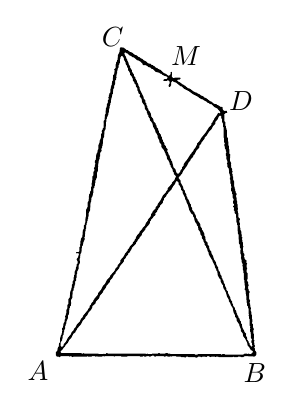
\begin{tikzpicture}[x=0.00612245cm,y=-0.00612245cm]
\fill[even odd rule] (228,257) -- (226,259) -- (225,267) -- (222,273) -- (221,283) -- (220,284) -- (220,286) -- (218,289) -- (218,292) -- (217,293) -- (217,300) -- (214,303) -- (215,305) -- (214,313) -- (212,315) -- (211,327) -- (210,328) -- (210,331) -- (209,332) -- (209,335) -- (208,336) -- (208,338) -- (207,339) -- (207,343) -- (206,344) -- (206,351) -- (204,353) -- (204,355) -- (203,356) -- (203,360) -- (202,361) -- (203,365) -- (201,367) -- (201,372) -- (199,375) -- (199,380) -- (198,381) -- (198,383) -- (197,384) -- (197,388) -- (196,389) -- (196,396) -- (195,397) -- (194,408) -- (192,410) -- (192,415) -- (193,416) -- (192,418) -- (192,424) -- (190,426) -- (190,428) -- (188,431) -- (189,435) -- (187,437) -- (187,444) -- (186,445) -- (186,447) -- (184,451) -- (184,454) -- (181,461) -- (181,469) -- (180,470) -- (179,476) -- (177,479) -- (176,490) -- (174,493) -- (174,497) -- (175,498) -- (175,500) -- (174,501) -- (174,505) -- (172,508) -- (173,510) -- (173,513) -- (171,516) -- (171,523) -- (169,525) -- (169,533) -- (168,534) -- (168,538) -- (167,539) -- (167,543) -- (168,545) -- (166,547) -- (166,554) -- (164,557) -- (164,560) -- (162,563) -- (161,576) -- (159,579) -- (159,588) -- (156,594) -- (156,608) -- (155,609) -- (155,612) -- (154,613) -- (154,621) -- (153,622) -- (153,625) -- (151,627) -- (151,634) -- (149,637) -- (148,650) -- (145,655) -- (145,658) -- (144,659) -- (144,666) -- (143,667) -- (144,670) -- (142,672) -- (142,680) -- (140,682) -- (136,682) -- (135,683) -- (136,685) -- (139,684) -- (141,686) -- (139,693) -- (136,697) -- (138,701) -- (138,706) -- (136,708) -- (136,712) -- (135,713) -- (134,719) -- (132,723) -- (132,729) -- (131,730) -- (131,734) -- (130,735) -- (130,740) -- (128,743) -- (128,748) -- (126,750) -- (126,756) -- (125,757) -- (125,760) -- (123,764) -- (122,776) -- (119,780) -- (119,790) -- (117,792) -- (117,799) -- (115,802) -- (115,809) -- (114,810) -- (114,813) -- (112,815) -- (113,820) -- (111,823) -- (111,827) -- (109,830) -- (108,838) -- (106,840) -- (106,843) -- (107,845) -- (106,846) -- (106,850) -- (105,851) -- (105,853) -- (103,856) -- (103,859) -- (102,860) -- (102,869) -- (100,871) -- (100,873) -- (99,874) -- (99,878) -- (97,881) -- (96,887) -- (93,890) -- (93,896) -- (95,899) -- (99,899) -- (100,900) -- (101,900) -- (103,898) -- (120,898) -- (121,899) -- (124,898) -- (128,900) -- (129,899) -- (157,899) -- (158,898) -- (160,899) -- (167,899) -- (168,898) -- (174,898) -- (175,899) -- (177,899) -- (178,898) -- (180,899) -- (189,899) -- (190,898) -- (192,898) -- (193,899) -- (195,898) -- (213,898) -- (214,899) -- (216,898) -- (228,898) -- (229,899) -- (241,899) -- (242,898) -- (267,898) -- (268,899) -- (273,899) -- (274,898) -- (276,898) -- (277,899) -- (280,899) -- (281,898) -- (286,898) -- (287,899) -- (289,899) -- (293,897) -- (296,897) -- (298,899) -- (300,899) -- (301,898) -- (317,898) -- (318,899) -- (320,899) -- (321,898) -- (324,898) -- (325,899) -- (330,899) -- (331,898) -- (333,899) -- (335,898) -- (342,898) -- (343,899) -- (352,899) -- (353,900) -- (360,900) -- (361,901) -- (362,901) -- (364,899) -- (367,899) -- (368,900) -- (382,900) -- (383,901) -- (386,901) -- (388,899) -- (393,899) -- (394,900) -- (396,900) -- (397,899) -- (403,899) -- (405,900) -- (408,898) -- (410,898) -- (414,900) -- (416,899) -- (423,899) -- (424,900) -- (426,899) -- (430,899) -- (431,900) -- (460,900) -- (461,899) -- (463,900) -- (470,900) -- (471,899) -- (476,899) -- (477,900) -- (482,900) -- (485,898) -- (505,899) -- (507,898) -- (509,895) -- (509,890) -- (506,886) -- (506,882) -- (505,881) -- (505,879) -- (506,878) -- (506,876) -- (505,875) -- (505,871) -- (504,870) -- (505,865) -- (503,863) -- (504,861) -- (504,852) -- (503,851) -- (503,844) -- (504,842) -- (502,838) -- (502,832) -- (500,830) -- (500,828) -- (501,827) -- (501,822) -- (500,821) -- (500,813) -- (499,812) -- (499,807) -- (497,803) -- (498,798) -- (497,797) -- (496,789) -- (495,788) -- (496,782) -- (494,780) -- (494,767) -- (495,766) -- (495,764) -- (493,762) -- (493,759) -- (492,758) -- (492,753) -- (493,752) -- (493,750) -- (492,749) -- (492,745) -- (490,742) -- (490,739) -- (491,738) -- (491,726) -- (489,724) -- (489,718) -- (490,717) -- (490,715) -- (489,714) -- (489,708) -- (490,706) -- (488,704) -- (489,700) -- (485,697) -- (485,694) -- (483,692) -- (484,690) -- (484,686) -- (482,684) -- (482,681) -- (481,680) -- (481,673) -- (482,672) -- (482,670) -- (481,669) -- (481,662) -- (480,661) -- (480,657) -- (479,656) -- (480,652) -- (478,649) -- (479,647) -- (478,645) -- (478,640) -- (476,636) -- (476,632) -- (475,631) -- (475,628) -- (474,627) -- (475,625) -- (475,622) -- (474,621) -- (474,616) -- (475,615) -- (475,613) -- (472,610) -- (472,602) -- (471,601) -- (471,598) -- (470,597) -- (471,591) -- (470,590) -- (470,583) -- (469,582) -- (469,576) -- (468,575) -- (468,569) -- (467,568) -- (467,564) -- (468,563) -- (468,561) -- (466,558) -- (466,556) -- (465,555) -- (465,551) -- (464,550) -- (464,547) -- (463,546) -- (463,536) -- (461,532) -- (461,526) -- (460,525) -- (460,521) -- (459,520) -- (459,517) -- (460,515) -- (459,514) -- (459,510) -- (457,507) -- (457,502) -- (456,501) -- (457,498) -- (454,492) -- (455,480) -- (453,478) -- (453,469) -- (452,468) -- (452,462) -- (451,461) -- (451,453) -- (450,452) -- (450,446) -- (448,443) -- (448,429) -- (447,428) -- (447,425) -- (446,424) -- (446,421) -- (445,420) -- (445,413) -- (443,411) -- (443,399) -- (442,397) -- (446,393) -- (449,393) -- (448,392) -- (448,389) -- (442,389) -- (440,387) -- (439,385) -- (439,382) -- (438,381) -- (435,381) -- (431,378) -- (428,377) -- (426,375) -- (423,375) -- (419,373) -- (416,370) -- (413,369) -- (404,362) -- (402,362) -- (399,359) -- (394,357) -- (392,355) -- (387,353) -- (385,351) -- (383,351) -- (379,349) -- (371,343) -- (367,342) -- (360,336) -- (359,336) -- (357,334) -- (355,334) -- (352,331) -- (345,327) -- (345,325) -- (346,324) -- (350,324) -- (352,322) -- (351,320) -- (340,320) -- (339,321) -- (336,321) -- (333,317) -- (334,315) -- (334,309) -- (333,308) -- (331,309) -- (331,313) -- (328,316) -- (326,316) -- (321,312) -- (319,312) -- (317,310) -- (316,310) -- (310,304) -- (305,302) -- (303,300) -- (301,300) -- (297,296) -- (296,296) -- (294,294) -- (292,294) -- (289,291) -- (286,291) -- (284,290) -- (281,287) -- (275,284) -- (272,281) -- (269,280) -- (267,278) -- (264,277) -- (261,274) -- (257,273) -- (251,268) -- (247,267) -- (242,263) -- (240,263) -- (234,258) -- cycle
(344,534) -- (348,538) -- (348,542) -- (350,544) -- (353,550) -- (353,553) -- (356,556) -- (356,559) -- (361,569) -- (362,574) -- (364,576) -- (364,578) -- (367,584) -- (370,595) -- (374,602) -- (378,605) -- (378,608) -- (380,611) -- (381,617) -- (383,621) -- (385,623) -- (386,627) -- (388,629) -- (389,636) -- (391,638) -- (393,642) -- (393,645) -- (396,649) -- (396,653) -- (399,657) -- (399,659) -- (402,664) -- (402,667) -- (405,670) -- (405,672) -- (407,675) -- (408,680) -- (410,683) -- (410,686) -- (413,692) -- (415,694) -- (416,697) -- (418,699) -- (418,701) -- (423,711) -- (423,713) -- (426,718) -- (426,720) -- (428,722) -- (429,730) -- (432,736) -- (435,739) -- (435,743) -- (438,749) -- (440,751) -- (440,755) -- (441,756) -- (441,758) -- (443,760) -- (446,766) -- (448,774) -- (452,781) -- (452,784) -- (455,788) -- (456,792) -- (460,798) -- (462,808) -- (465,813) -- (465,816) -- (468,820) -- (468,824) -- (474,833) -- (474,835) -- (477,842) -- (477,846) -- (481,851) -- (482,857) -- (486,862) -- (490,870) -- (491,876) -- (494,879) -- (498,886) -- (500,886) -- (502,888) -- (502,890) -- (498,894) -- (495,894) -- (494,893) -- (492,893) -- (491,894) -- (489,893) -- (485,893) -- (482,895) -- (444,895) -- (443,894) -- (439,894) -- (438,895) -- (436,895) -- (435,894) -- (388,894) -- (387,895) -- (382,895) -- (381,894) -- (331,894) -- (330,893) -- (326,893) -- (325,892) -- (321,892) -- (320,893) -- (309,893) -- (308,892) -- (306,892) -- (305,893) -- (293,893) -- (292,894) -- (284,894) -- (283,893) -- (281,894) -- (279,893) -- (201,893) -- (200,892) -- (198,892) -- (196,894) -- (194,894) -- (193,893) -- (191,894) -- (182,894) -- (181,893) -- (152,893) -- (151,892) -- (149,893) -- (147,893) -- (146,892) -- (105,892) -- (103,890) -- (103,888) -- (108,883) -- (108,882) -- (112,878) -- (113,875) -- (118,870) -- (121,864) -- (125,860) -- (129,852) -- (134,848) -- (134,846) -- (136,844) -- (137,841) -- (145,832) -- (149,824) -- (154,819) -- (154,817) -- (158,813) -- (161,807) -- (166,802) -- (169,796) -- (169,794) -- (175,789) -- (176,785) -- (182,779) -- (184,775) -- (184,773) -- (191,765) -- (191,763) -- (196,757) -- (198,752) -- (205,744) -- (206,740) -- (210,736) -- (213,730) -- (217,726) -- (217,724) -- (224,716) -- (226,711) -- (233,703) -- (234,701) -- (234,698) -- (238,694) -- (239,691) -- (243,687) -- (243,685) -- (247,682) -- (247,680) -- (249,678) -- (251,673) -- (259,665) -- (259,663) -- (261,661) -- (263,657) -- (267,653) -- (267,651) -- (271,647) -- (272,643) -- (279,635) -- (279,633) -- (287,624) -- (288,622) -- (288,619) -- (290,617) -- (290,615) -- (295,610) -- (295,609) -- (300,605) -- (299,602) -- (303,598) -- (303,596) -- (305,594) -- (306,591) -- (309,588) -- (309,586) -- (314,581) -- (315,579) -- (315,576) -- (317,574) -- (317,571) -- (322,566) -- (323,563) -- (326,560) -- (326,559) -- (333,552) -- (334,549) -- (336,547) -- (336,546) -- (340,541) -- (342,536) -- cycle
(433,399) -- (435,399) -- (437,401) -- (436,404) -- (438,406) -- (438,412) -- (440,416) -- (440,422) -- (441,423) -- (441,444) -- (442,445) -- (442,454) -- (444,456) -- (443,458) -- (443,462) -- (444,463) -- (444,467) -- (446,470) -- (446,473) -- (447,474) -- (447,476) -- (446,477) -- (446,482) -- (447,483) -- (447,489) -- (449,493) -- (449,497) -- (448,499) -- (449,500) -- (449,505) -- (452,509) -- (453,520) -- (454,521) -- (454,524) -- (455,525) -- (455,527) -- (454,528) -- (454,531) -- (455,532) -- (455,539) -- (457,542) -- (457,546) -- (458,547) -- (457,549) -- (457,555) -- (459,558) -- (459,561) -- (460,562) -- (460,569) -- (462,572) -- (462,575) -- (461,576) -- (461,581) -- (463,583) -- (463,585) -- (461,587) -- (461,588) -- (463,590) -- (463,593) -- (462,595) -- (464,597) -- (464,601) -- (467,604) -- (468,621) -- (469,622) -- (469,625) -- (470,626) -- (470,638) -- (471,639) -- (471,644) -- (472,645) -- (473,664) -- (475,667) -- (475,672) -- (477,676) -- (476,678) -- (476,685) -- (477,686) -- (477,689) -- (478,690) -- (477,695) -- (478,696) -- (479,704) -- (481,707) -- (480,711) -- (481,712) -- (481,719) -- (482,720) -- (482,725) -- (483,726) -- (483,739) -- (484,740) -- (484,745) -- (485,746) -- (485,751) -- (486,752) -- (486,757) -- (485,758) -- (485,760) -- (487,762) -- (487,765) -- (488,766) -- (487,767) -- (488,768) -- (487,769) -- (488,770) -- (489,787) -- (490,788) -- (490,793) -- (492,795) -- (492,798) -- (493,799) -- (493,810) -- (494,811) -- (493,814) -- (494,815) -- (494,820) -- (495,821) -- (495,834) -- (497,837) -- (496,839) -- (497,841) -- (496,843) -- (496,847) -- (497,848) -- (497,851) -- (498,852) -- (498,861) -- (500,863) -- (500,865) -- (499,866) -- (499,870) -- (500,871) -- (501,877) -- (499,879) -- (495,874) -- (495,872) -- (493,870) -- (493,868) -- (490,864) -- (490,860) -- (487,855) -- (488,852) -- (484,848) -- (484,846) -- (480,839) -- (480,837) -- (479,836) -- (479,832) -- (477,830) -- (477,826) -- (475,824) -- (474,820) -- (472,818) -- (472,816) -- (469,812) -- (469,810) -- (468,809) -- (467,804) -- (465,802) -- (464,797) -- (461,794) -- (461,792) -- (459,788) -- (459,785) -- (457,783) -- (455,779) -- (455,777) -- (450,767) -- (450,764) -- (447,761) -- (447,758) -- (444,752) -- (444,750) -- (441,745) -- (441,742) -- (439,740) -- (439,738) -- (437,735) -- (437,732) -- (435,730) -- (433,723) -- (431,721) -- (431,719) -- (430,718) -- (430,714) -- (428,712) -- (426,708) -- (425,703) -- (421,697) -- (419,690) -- (416,685) -- (416,682) -- (412,677) -- (412,675) -- (411,674) -- (411,670) -- (408,667) -- (408,663) -- (404,659) -- (403,650) -- (401,648) -- (401,644) -- (398,638) -- (396,636) -- (396,633) -- (393,629) -- (393,625) -- (390,620) -- (387,617) -- (387,615) -- (384,611) -- (383,605) -- (381,603) -- (381,601) -- (376,595) -- (376,591) -- (373,587) -- (373,583) -- (371,581) -- (370,577) -- (368,573) -- (366,571) -- (366,569) -- (364,566) -- (364,563) -- (361,558) -- (361,555) -- (358,552) -- (357,547) -- (352,538) -- (352,534) -- (348,529) -- (348,527) -- (355,519) -- (357,514) -- (365,503) -- (369,495) -- (372,492) -- (373,489) -- (378,484) -- (378,482) -- (381,479) -- (385,471) -- (390,466) -- (391,464) -- (391,461) -- (394,458) -- (395,455) -- (402,446) -- (402,444) -- (406,440) -- (411,432) -- (416,427) -- (419,421) -- (423,417) -- (424,415) -- (424,412) -- (429,406) -- (431,401) -- cycle
(231,275) -- (234,279) -- (234,282) -- (238,289) -- (238,292) -- (241,296) -- (241,298) -- (243,301) -- (243,305) -- (245,307) -- (247,311) -- (247,314) -- (250,317) -- (253,323) -- (253,326) -- (256,330) -- (256,332) -- (259,335) -- (259,338) -- (262,342) -- (262,346) -- (264,349) -- (264,352) -- (268,355) -- (267,359) -- (271,364) -- (272,371) -- (277,378) -- (278,385) -- (282,390) -- (282,393) -- (283,394) -- (283,396) -- (285,398) -- (285,401) -- (288,405) -- (288,408) -- (293,414) -- (295,422) -- (299,429) -- (300,434) -- (302,436) -- (304,440) -- (304,443) -- (308,451) -- (308,454) -- (312,459) -- (312,464) -- (317,470) -- (319,474) -- (319,476) -- (321,478) -- (321,480) -- (323,483) -- (324,489) -- (326,491) -- (329,497) -- (329,500) -- (331,502) -- (331,504) -- (335,510) -- (336,515) -- (338,517) -- (338,520) -- (342,524) -- (342,526) -- (339,533) -- (334,538) -- (334,540) -- (325,550) -- (325,553) -- (323,555) -- (321,559) -- (315,565) -- (310,575) -- (304,583) -- (304,585) -- (300,589) -- (300,592) -- (294,598) -- (293,601) -- (291,603) -- (290,608) -- (284,615) -- (284,617) -- (280,622) -- (278,627) -- (274,631) -- (271,636) -- (267,640) -- (266,643) -- (262,647) -- (259,652) -- (259,654) -- (257,656) -- (256,659) -- (253,662) -- (253,664) -- (247,670) -- (245,674) -- (242,677) -- (242,679) -- (237,685) -- (234,691) -- (227,699) -- (227,703) -- (221,710) -- (221,712) -- (217,716) -- (215,721) -- (206,731) -- (205,734) -- (199,740) -- (195,748) -- (191,752) -- (187,760) -- (181,767) -- (180,771) -- (173,779) -- (173,780) -- (171,782) -- (171,784) -- (167,788) -- (166,791) -- (163,794) -- (163,797) -- (161,799) -- (159,803) -- (149,815) -- (149,817) -- (145,821) -- (143,826) -- (137,832) -- (134,838) -- (131,841) -- (130,844) -- (126,848) -- (124,853) -- (118,860) -- (114,868) -- (109,874) -- (109,876) -- (106,879) -- (105,879) -- (103,877) -- (103,869) -- (106,865) -- (106,862) -- (107,861) -- (107,856) -- (109,853) -- (109,849) -- (110,848) -- (110,845) -- (112,841) -- (112,836) -- (113,835) -- (113,833) -- (115,829) -- (115,826) -- (118,819) -- (118,814) -- (120,811) -- (121,799) -- (122,798) -- (122,795) -- (124,793) -- (124,790) -- (125,789) -- (124,788) -- (125,787) -- (124,786) -- (124,782) -- (127,777) -- (128,763) -- (130,761) -- (130,757) -- (131,756) -- (132,750) -- (133,749) -- (133,743) -- (135,741) -- (135,736) -- (136,735) -- (136,728) -- (137,727) -- (137,723) -- (140,717) -- (140,710) -- (143,704) -- (142,696) -- (143,695) -- (144,686) -- (146,683) -- (147,670) -- (149,668) -- (149,665) -- (150,664) -- (150,662) -- (153,655) -- (152,651) -- (153,650) -- (154,639) -- (155,638) -- (155,634) -- (156,633) -- (156,626) -- (157,625) -- (157,622) -- (158,621) -- (158,618) -- (159,617) -- (159,614) -- (160,613) -- (160,609) -- (161,608) -- (161,601) -- (164,595) -- (165,579) -- (166,578) -- (167,569) -- (169,566) -- (170,560) -- (171,559) -- (171,550) -- (173,548) -- (173,545) -- (174,544) -- (174,539) -- (175,538) -- (175,534) -- (178,527) -- (178,518) -- (180,514) -- (180,505) -- (181,504) -- (180,501) -- (181,500) -- (182,492) -- (184,488) -- (184,484) -- (185,483) -- (185,476) -- (188,472) -- (187,468) -- (189,465) -- (189,462) -- (190,461) -- (191,447) -- (193,443) -- (194,430) -- (196,427) -- (196,422) -- (197,421) -- (197,412) -- (198,411) -- (198,406) -- (199,405) -- (199,403) -- (202,396) -- (202,393) -- (203,392) -- (203,386) -- (204,385) -- (205,377) -- (206,376) -- (206,373) -- (207,372) -- (207,366) -- (208,365) -- (208,362) -- (209,361) -- (210,355) -- (211,354) -- (212,344) -- (214,341) -- (214,337) -- (216,333) -- (216,326) -- (218,324) -- (218,321) -- (219,320) -- (218,316) -- (219,315) -- (219,312) -- (220,311) -- (220,306) -- (221,305) -- (221,302) -- (223,299) -- (223,294) -- (225,292) -- (225,290) -- (226,289) -- (226,282) -- (227,281) -- (227,278) -- (229,275) -- cycle
(237,267) -- (239,269) -- (242,270) -- (246,274) -- (249,275) -- (253,278) -- (255,278) -- (262,284) -- (264,284) -- (266,286) -- (268,286) -- (273,291) -- (273,293) -- (274,294) -- (279,294) -- (283,296) -- (285,298) -- (289,299) -- (292,302) -- (294,302) -- (300,308) -- (308,310) -- (310,312) -- (312,312) -- (314,314) -- (320,317) -- (322,317) -- (325,320) -- (325,321) -- (323,323) -- (319,323) -- (317,324) -- (316,326) -- (317,327) -- (323,327) -- (324,326) -- (327,326) -- (329,328) -- (329,332) -- (327,336) -- (327,338) -- (328,339) -- (330,339) -- (332,336) -- (332,331) -- (333,329) -- (335,327) -- (336,327) -- (338,329) -- (342,330) -- (352,338) -- (354,338) -- (359,343) -- (369,348) -- (377,354) -- (387,359) -- (392,363) -- (396,365) -- (398,365) -- (400,367) -- (406,370) -- (408,372) -- (411,373) -- (413,375) -- (416,375) -- (422,381) -- (428,384) -- (435,392) -- (432,395) -- (431,393) -- (428,396) -- (428,397) -- (422,405) -- (421,408) -- (419,410) -- (418,413) -- (416,415) -- (416,418) -- (411,423) -- (404,434) -- (395,445) -- (391,452) -- (386,457) -- (386,459) -- (383,465) -- (379,470) -- (378,473) -- (375,476) -- (375,477) -- (372,480) -- (365,491) -- (360,497) -- (358,501) -- (358,503) -- (355,506) -- (355,509) -- (352,512) -- (351,516) -- (347,520) -- (346,520) -- (343,517) -- (341,510) -- (337,506) -- (334,494) -- (332,492) -- (332,490) -- (330,487) -- (329,482) -- (327,480) -- (326,476) -- (324,473) -- (325,469) -- (322,466) -- (321,462) -- (318,459) -- (318,456) -- (315,452) -- (315,450) -- (313,447) -- (313,444) -- (311,441) -- (311,439) -- (307,434) -- (307,431) -- (305,429) -- (305,426) -- (302,423) -- (302,420) -- (300,417) -- (300,415) -- (296,411) -- (295,406) -- (291,401) -- (290,395) -- (288,391) -- (285,388) -- (285,385) -- (283,383) -- (283,380) -- (281,377) -- (281,374) -- (279,372) -- (279,368) -- (275,363) -- (275,360) -- (267,344) -- (267,341) -- (264,336) -- (264,334) -- (261,329) -- (261,327) -- (258,322) -- (258,320) -- (255,317) -- (255,314) -- (251,308) -- (251,305) -- (247,299) -- (247,297) -- (244,292) -- (244,290) -- (241,284) -- (241,282) -- (239,280) -- (239,278) -- (236,273) -- (235,269) -- cycle;
\node[inner sep=0pt] at (211,236) {$C$};
\node[inner sep=0pt] at (363,276) {$M$};
\node[inner sep=0pt] at (477,369) {$D$};
\node[inner sep=0pt] at (56,929) {$A$};
\node[inner sep=0pt] at (506,933) {$B$};
\end{tikzpicture}
\\[3pt]Fig. 3.\end{minipage}
\end{center}
Um Euklids Beweis I. 7 stringent zu machen, ohne vorher die Ebene anders definirt
zu haben, als »die Fläche, welche durch Umdrehung einer Geraden um eine Axe
[entsteht], mit der sie rechte Winkel macht«, muss man in der 2. und 3. Figur $CD$
in $M$ halbiren und durch $M$ ein Planum legen, gegen welches $CD$ normal ist,
\emph{in} diesem liegen $A$ und $B$, während $C$ und $D$ ausserhalb liegen. Es
braucht also nur bewiesen zu werden, dass kein Punkt von $AD$ und $BC$ ($AD$ für
die Fig. 2 indefinite verlängert) in dem Planum liegt, was keine Schwierigkeit
hat. Es folgt dann von selbst, dass die Voraussetzung absurd ist, sobald $AD$ und
$BC$ einander schneiden.

